% --------------------------------------------------------------------------------------
%                   LATEX TEMPLATE FOR DISSERTATION (HONS)
% --------------------------------------------------------------------------------------
\documentclass[11pt]{book}

\usepackage{amsfonts, amsmath, amssymb}  
\usepackage{times}

%\usepackage[backref=page,pagebackref=true,linkcolor = blue,citecolor = red]{hyperref}
%\usepackage[backref=page]{backref}

\usepackage{graphicx}
\DeclareGraphicsExtensions{.pdf,.png,.jpg}

\setlength{\oddsidemargin}{1.5cm}
\setlength{\evensidemargin}{0cm}
\setlength{\topmargin}{1mm}
\setlength{\headheight}{1.36cm}
\setlength{\headsep}{1.00cm}
%\setlength{\textheight}{20.84cm}
\setlength{\textheight}{19cm}
\setlength{\textwidth}{14.5cm}
\setlength{\marginparsep}{1mm}
\setlength{\marginparwidth}{3cm}
\setlength{\footskip}{2.36cm}


\begin{document}
\pagestyle{empty}

%: ----------------------------------------------------------------------
%:                  TITLE PAGE: name, degree,..
% ----------------------------------------------------------------------

\begin{center}

\vspace{1cm}

%%% Type the thesis title below%%%%%%%%%%%%%%%%
{\Huge         High-Performance Hadoop Map/Reduce R Interface Enhancement}

\vspace{25mm} 


\includegraphics[width=3.5cm]{logo}

 \vspace{35mm}

%%%%%Type Your Name Below%%%%%%%%%%%%
{\Large       Noah Zhang}

	\vspace{1ex}

Department of Statistics

The University of Auckland

	\vspace{5ex}

 %%%%%Typing Your Supervisors Name Below%%%%%%%%%%%%
Supervisor:             Simon Urbanek

	\vspace{30mm}

A dissertation submitted in partial fulfillment of the requirements for the degree of BSc(Hons) in Statistics, The University of Auckland, 2020.

\end{center}

\newpage


%: --------------------------------------------------------------
%:                  FRONT MATTER:  abstract,..
% --------------------------------------------------------------
\chapter*{Abstract}       
\setcounter{page}{1}
\pagestyle{headings}
% \pagenumbering{roman}

\addcontentsline{toc}{chapter}{Abstract}


 Put your abstract  here.  The abstract should contain a brief summary of the aim, methodologies, 
finding and conclusions of the dissertation.  The abstract should normally be fewer than 350 words.


Big data is concern massive amount, complex, growing data set from multiple autonomous sources. It has to deal with large
and complex dataset that can be structured, semi-structured or unstructured and will typically not fit into memory to be processed.
MapReduce is a programming model for processing large datasets distributed on a large clusters.A rapid growth of data in recent time,
Industries and academia required an intelligent data analysis tool that would be helpful to satisfy the need to analysis a large amount of
data. MapReduce framework is basically designed to compute data demanding applications to support effective decision making. Since
its introduction, remarkable research efforts have been put to make it more familiar to the users subsequently utilized to support the
execution of enormous data intensive applications. This survey paper highlights and investigates various applications using recent
MapReduce models.





%: --------------------------------------------------------------
%:                  END:  abstract
% --------------------------------------------------------------


%: ----------------------- contents ------------------------
\setcounter{secnumdepth}{3} % organisational level that receives a numbers
\setcounter{tocdepth}{3}    % print table of contents for level 3
\tableofcontents            % print the table of contents
% levels are: 0 - chapter, 1 - section, 2 - subsection, 3 - subsection

%: --------------------------------------------------------------
%:                  MAIN DOCUMENT SECTION
% --------------------------------------------------------------
	
\chapter{Introduction}%    \chapter{}  = level 1, top level

A thesis should always have an introduction.  The purpose is to describe the general subject area, state the research problem of interest, outline the main results of the thesis, and put the results in context with the wider subject area and its applications.

The main body of the text must be divided into a logical scheme which  is followed consistently throughout the work.  
 It usually starts with an introduction chapter  and ends with  a conclusion chapter. See, for example, the table of contents on page 3. 

There is strict  35-page limit  for an applied mathematics dissertation,  including  the references  but excluding  appendices. 

\chapter{Concept of Big Data}

Big data concerns huge amounts, complex and diverse sets of information that is growing at ever-increasing rates. The size of the data suggest that we will need to deviate from the traditional processing methodologies and to adapt an inexpensive and efficient way through distributed/parallel computing.\\

Today, we can find upwards of 800 million webpages providing documentation on big data. Enthusiasts believe that Big Data is the next big thing after Cloud [1]. 

\section{Characteristics of Big Data}

The concept of big data is generally vague without a formal definition, however the general consensus is that there are specific attributes that define big data The four characteristics of big data are Volume, Velocity, Variety and Veracity [2]. 

\begin{center}
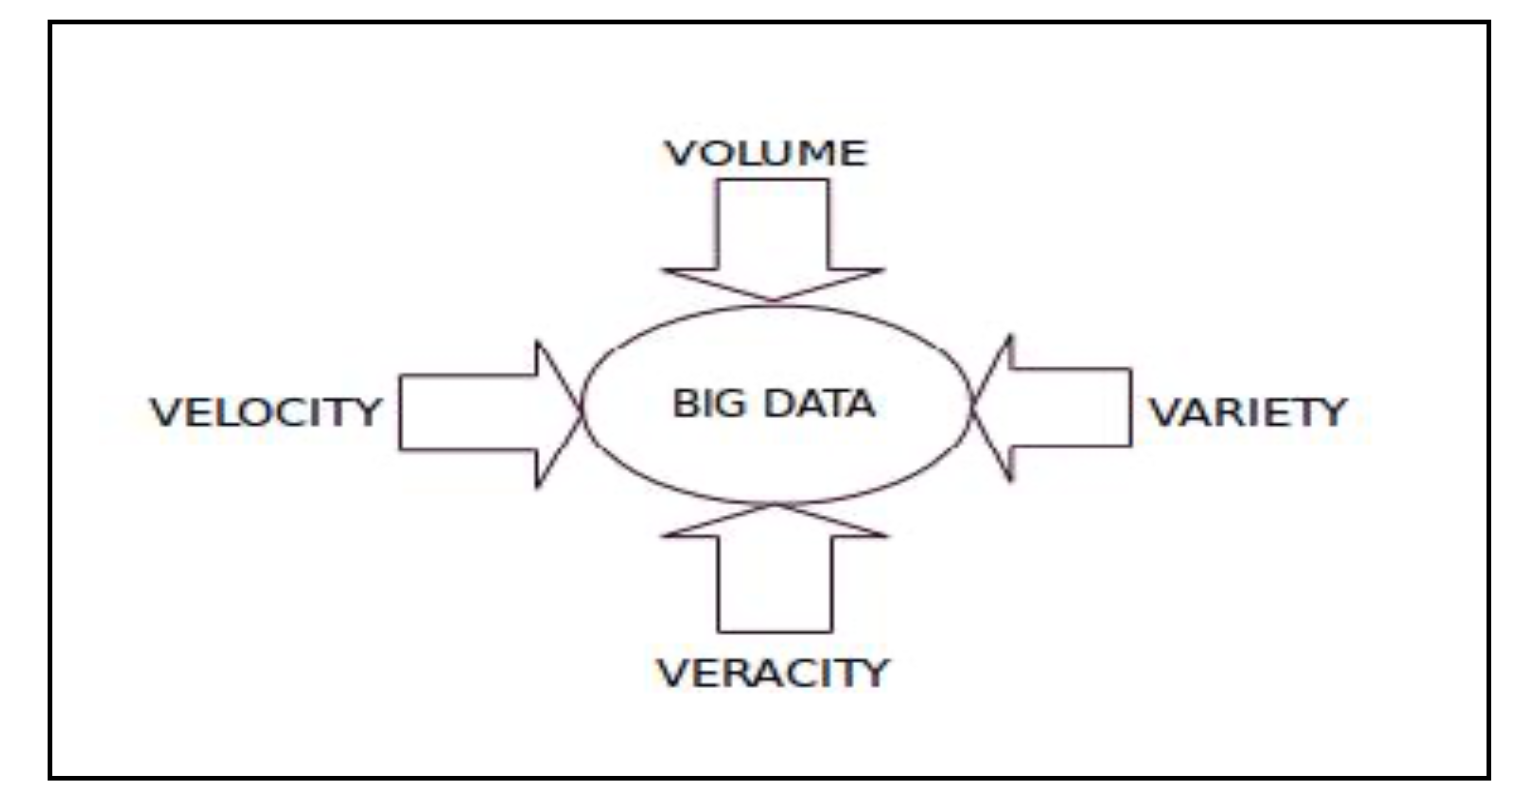
\includegraphics[width=10cm]{4vbd}\\
\end{center}

The main characteristic that makes data “big” is its sheer volume. According to estimates by IBM, we can expect at least 40 Zettabytes (43 Trillion Gigabytes) of data to be created in 2020 [3]. The volume of data sets being processed and analysed has reached sizes larger than terabytes and even petabytes. This suggests that data sets these days are becoming too large to process within a single desktop machine/processor. \\

Velocity is the speed at which data is generated. High velocity data is generated with such a pace that it may require certain distributed processing techniques. Good examples of high velocity data includes social media posts.\\

Variety is the source of the data which can be found in different forms such as text, numerical, images, audio and video records. The variety in the data will require distinct processing capabilities or algorithms to handle different formats. \\

Veracity is the quality of the data. Information may be volatile or incomplete seen in low veracity data sets containing a high percentage of meaningless data referred to as noise. On the other hand, high veracity data hold records that are valuable to analyse and contribute in a meaningful way to the overall results.

\section{Structure of Big Data} 

Big data can be categorised as structured or unstructured.\\
 
Structured data is usually stored and managed in relational databases with predefined data models. Examples of relational database applications with structured data include customer information, sales transactions, airline reservations systems, and billing systems. This type of structured data within relational databases can be accessed using Structured Query language (SQL).\\
 
Unstructured data, in contrast, has its internal structure but it is not structured through pre-defined data models or schema. As it may comes in many different formats, it cannot be stored in relational databases which also becomes a real challenge for systems to process and analyse. The unstructured data may be stored within non-relational databases like NoSQL.

\chapter{The Hadoop Framework}

At present, with data being generated at an exponential rate, there is the need to deploy data intensive application and storage clusters in order to keep up with the amount of data. To handle such problem, Google introduced the MapReduce model for distributed computing based on Java. This system is implemented through Apache Hadoop which is an open source software framework. This framework offers reliable, scalable, parallel and distributed computing scaling up from a single server to a network of multiple computers[4]. Apache Hadoop was developed with the purpose of having a data store that allow organisations to leverage big data analytics with cost efficiency in mind.\\

%There are two main components of the Hadoop Framework: Storage and Processing

\section{Hadoop Architecture}

Hadoop follows a master/slave architecture design for data storage and distributed data processing using HDFS and MapReduce respectively. The master node for data storage is NameNode while the master node for parallel processing is the Job Tracker. The slave nodes are comprised of other machines in the Hadoop cluster which stores the data and performs the computations. Each slave node have a DataNode and a TaskTracker that synchronises the process respectively. \\

\begin{center}
 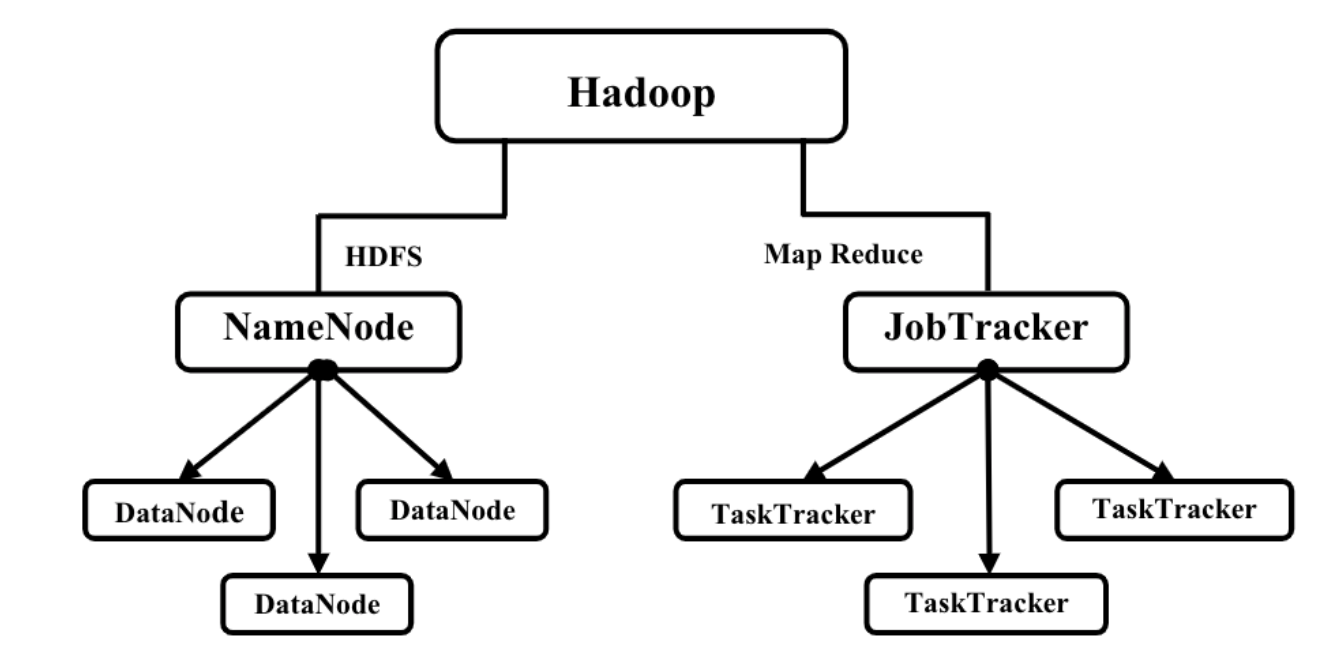
\includegraphics[width=10cm]{hadoop}\\
 \end{center}

The Hadoop system can be set up via cloud or locally. The cluster we will be running is a set up of 8 virtual machines.

\section{Storage - HDFS}

The storage component of the Hadoop architecture is known as the Hadoop Distributed File System (HDFS). The NameNode runs on the master node and manages metadata about the file system in a file named fsimage. This metadata is cached in main memory to provide faster access to the clients on read/write requests. The NameNode controls also manages the slaves by splitting files into chunks (default 64 megabytes) and distributing them across each DataNode in the cluster. The DataNodes are primary storage elements of HDFS where chunks of data are stored and replicated according to the instructions from the NameNode. Secondary NameNode is to periodically read the file system, log changes and applying them to the fsimage file. This will enable the NameNode to boot faster.\\

The main advantages of HDFS is data locality and fault tolerance. Data locality allow the nodes to manipulate the data they have access to which results in faster and more efficient processing while handling faults through the process of replicating files across each slave node[4].\\

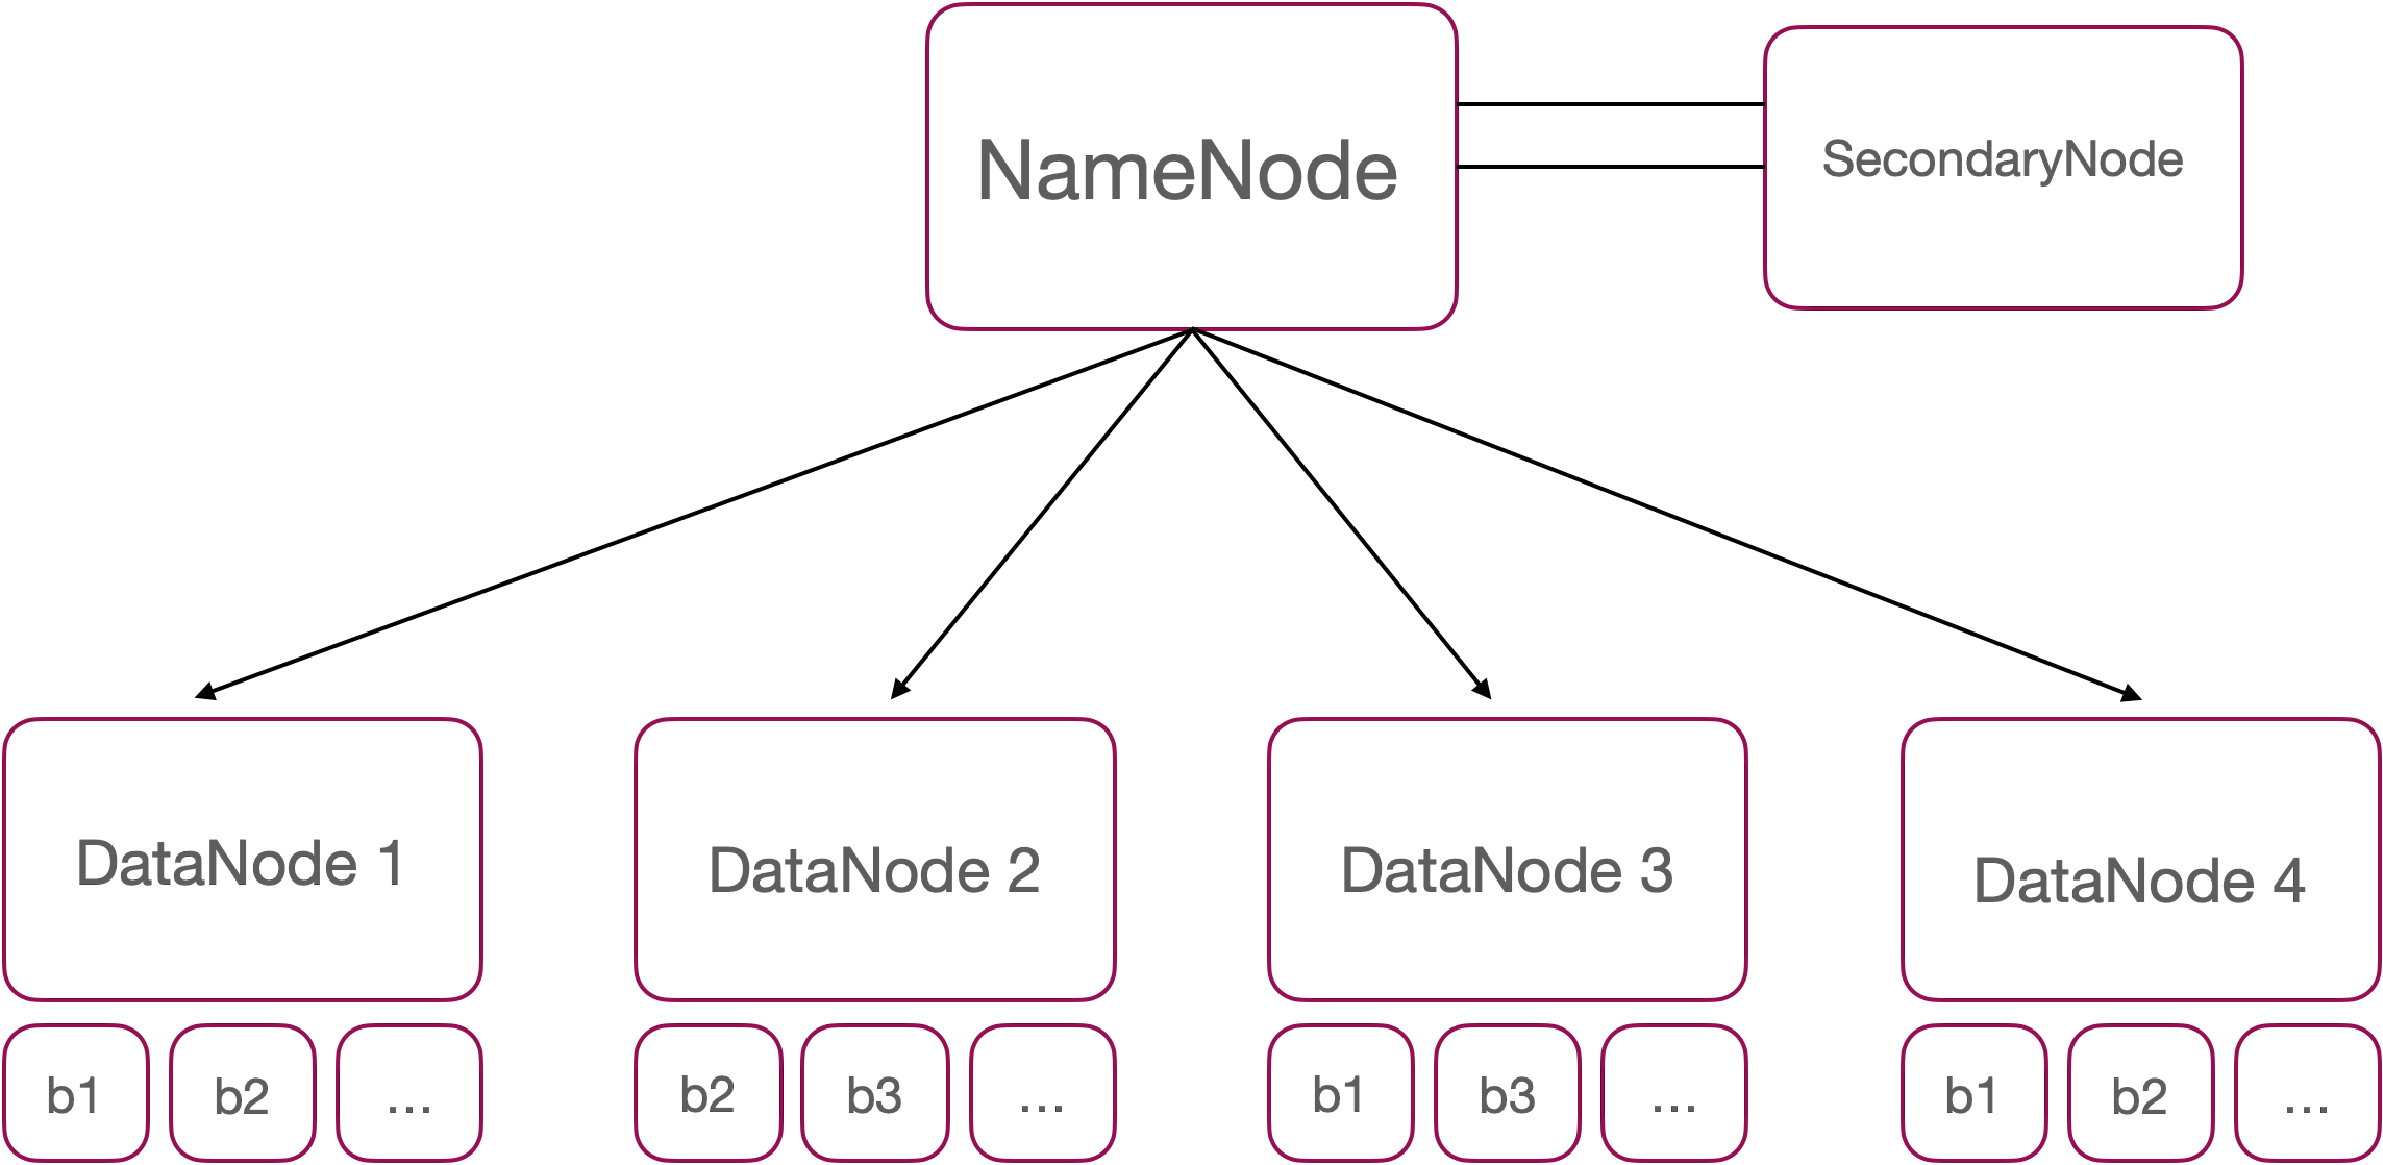
\includegraphics[width=8cm]{hdfs}

\section{Processing - MapReduce}

The processing component of the Hadoop architecture is know as MapReduce based on Java. MapReduce is used to process and analyse large data sets in parallel on a collective group of computers known as a cluster. In a MapReduce job, the input is broken down into multiple chunks which are processed by the map phase and then the output of the map phase is passed as input to the reduce phase. The input and output files are stored in the file system, while the output of the map phase (known as intermediate results) are only stored temporarily in the process.\\

The MapReduce framework operates on key-value pairs, which means that that the input to each phase are pairs of keys and values associated with its key. In addition, the user is also required to specify two scripts/functions: the mapper and the reducer. As the process runs in parallel, the reduce task on specific nodes may begin once its map tasks is complete rather than waiting on all map tasks to complete. \\


\includegraphics[width=8cm]{keyvalue}

Similar to HDFS, the MapReduce process also utilises the master/slave architecture in which the JobTracker runs on the master node while the TaskTracker runs on each slave node. \\

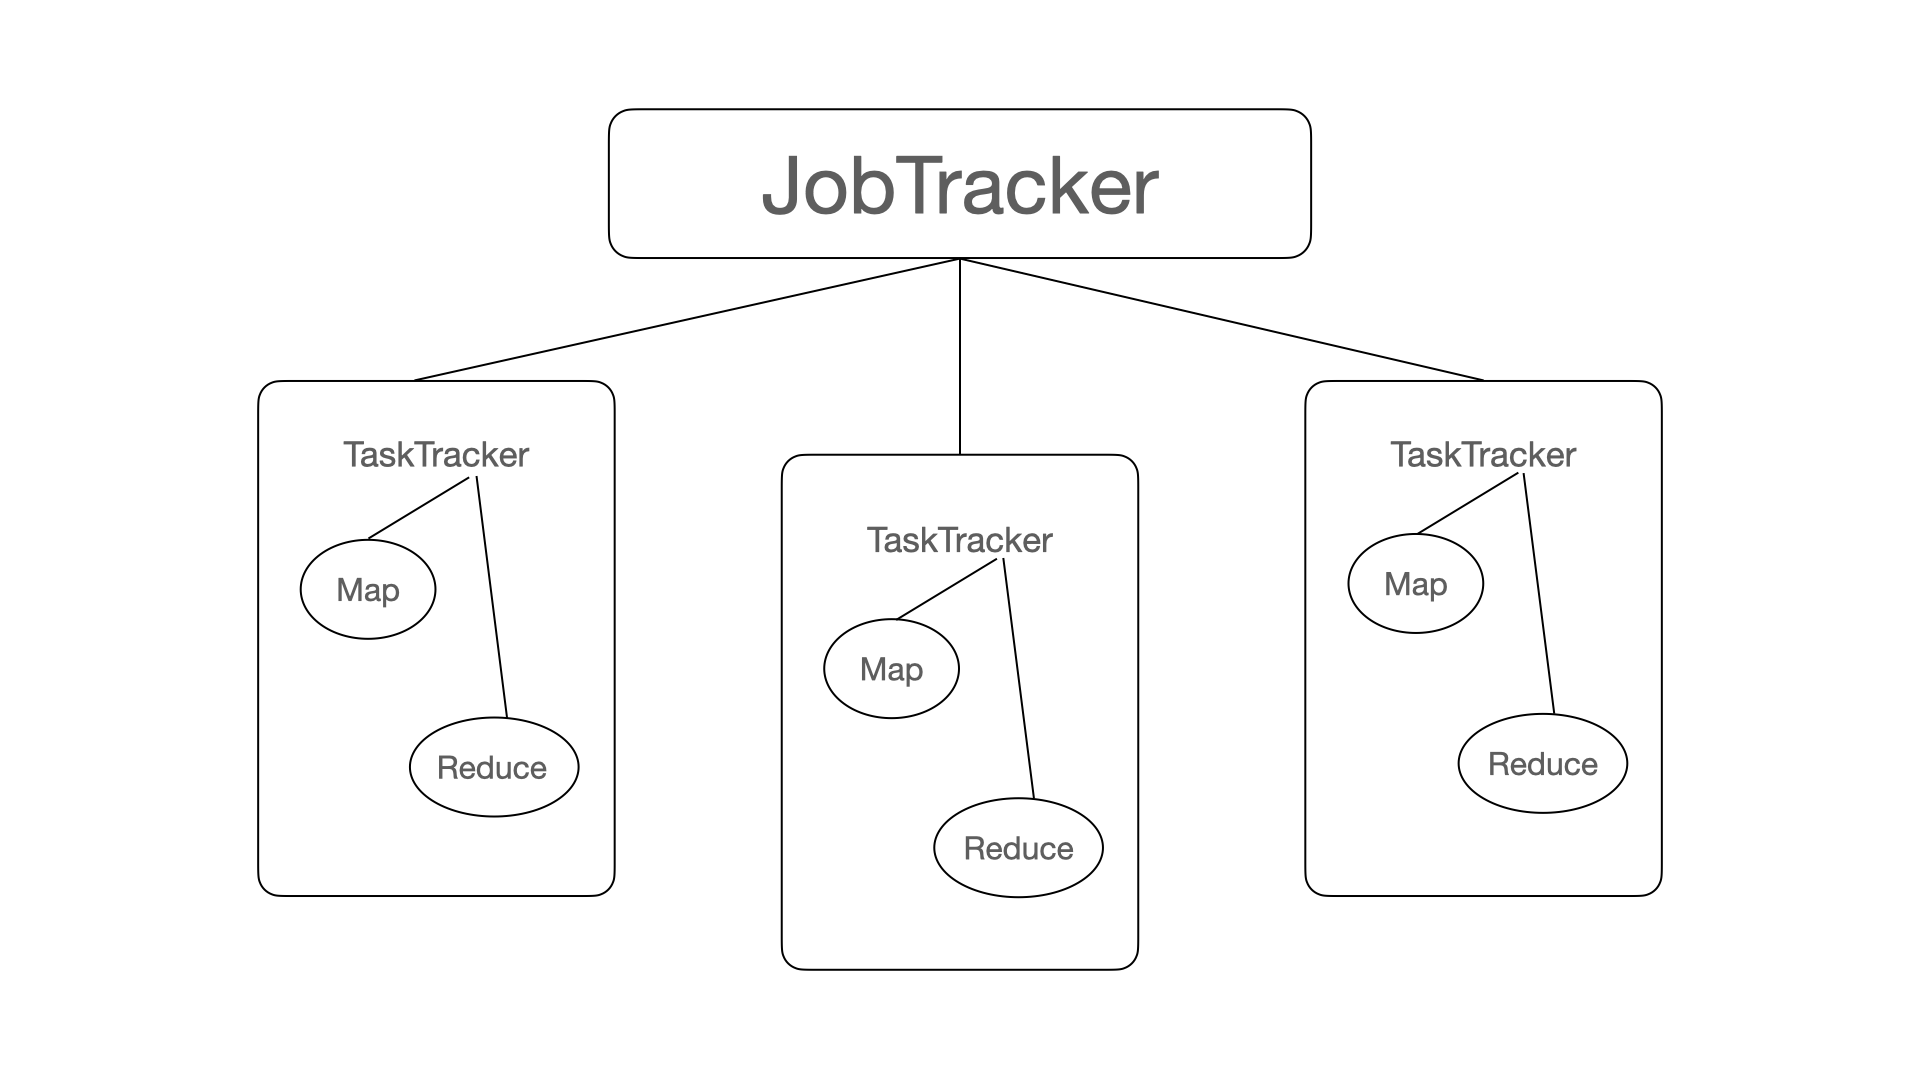
\includegraphics[width=8cm]{jobtracker}

The JobTracker monitors the MapReduce tasks carried out by the TaskTracker running on the slave nodes. The user will only interact with the master node by submitting jobs to the JobTracker. The JobTracker then locates and submits the jobs to the TaskTracker. The slave nodes are monitored by the JobTracker through heartbeat signals to determine whether a node has failed. The JobTracker is a point of failure for the Hadoop MapReduce service and if it goes down, all jobs will be stopped. \\

The TaskTracker runs on the slave nodes in a cluster and receives jobs from the JobTracker to execute the MapReduce tasks. Each TaskTracker has an allocation of task slots which indicate the number of tasks it can accept. The JobTracker will delegate jobs to the TaskTracker based on the number of available/empty slots while the TaskTracker will periodically send heartbeat signals to inform the JobTracker of any issues. TaskTracker failure is not considered fatal as tasks can be reallocated to another node when it becomes unresponsive.\\

\chapter{Hadoop Streaming}

Hadoop streaming is a utility that comes with the Hadoop distribution which allow users to create and run MapReduce jobs to be executed in the Hadoop cluster using other languages. By default the Hadoop MapReduce framework is written in Java but it utilizes Unix streams to pipe between Hadoop and our MapReduce program so we can use any language which can read standard input and write to standard output for our MapReduce program. MapReduce programs can be written in mutiple languages such as R, Python, Perl, PHP, C++, etc. The utility is packed in a JAR file. 

\section{Purpose}

Using the utility, we can create executable scripts to run MapReduce Jobs. Furthermore, we can create executable scripts to run the mapper and reducer functions which are passed to Hadoop streaming. The utility creates map and reduce jobs and submits them to the cluster which can then be monitored, thus enabling a person to write MapReduce job in the language of their choice without having any knowledge of Java.

\section{Syntax}

The syntax below can be used to run MapReduce jobs written in a different language to process data using the Hadoop MapReduce framework.\\

\begin{verbatim}
$HADOOP_HOME/bin/hadoop jar $HADOOP_HOME/hadoop-streaming.jar 
    -input myInputDirs 
    -output myOutputDir 
    -mapper /bin/cat 
    -reducer /usr/bin/wc
\end{verbatim}

The input command is used to provide the directory fo the input which the output command is used to provide the output directory. The mapper command is used to specify the executable mapper class while the reducer command is used to specify the executable reducer class.

The mapper command is used to specify the executable mapper class while the reducer command is used to specify the executable reducer class.

\section{How it Works}

Let us now explore how Hadoop streaming works.\\


\includegraphics[width=14cm]{streaming}\\

The mapper and reducer are scripts/functions created by the user that reads in the input line by line from standard input and returns the output to standard output. If the mapper script/function is specified, the mapper will converts the inputs into lines and converts the lines to the standard input which feeds into the mapper. In the process, the mapper converts each line into a key and value pair returned as standard output. If the reducer script/function is specified, the reducer then draws the line-oriented key value pairs from the mapper as standard input and converts each line collected into a key/value pair. This is then emitted to standard output. 

For both the mapper and the reducer, first entry of the line is the key followed by the value which is separate by a tab character. If there is no tab character in the line, then the entire line is considered as the key and the value is considered null. 

\section{Advantages}

1. Availability - the utility comes with the Hadoop distribution hence does not require further installation of softwares.\\
2. Learning - relatively easy to learn as it requires basic unix coding.\\
3. Reduce Development Time - it is much quicker to write mapper and reducer scripts/functions whereas using native Java MapReduce application is more complex as it requires the application to be complied, packaged, and exporting the JAR file.\\
4. Faster Conversion - it takes very little time to convert data from one format to another using Hadoop streaming especially when the input and output formats are specified.\\
5. Testing - input and output data can be tested quickly by using it with Unix or command line tools.

\chapter{MapReduce Framework}

We have already identified that MapReduce is a software framework and programming model in the Hadoop Architecture which is used for processing large amounts of data. It it based on Java but also has the capability to run in languages other than JAVA through the Hadoop streaming utility. Let us know explore how the MapReduce process works.

The complete process typically consists of four operations namely, splitting, mapping, shuffling and reducing.\\

1. Splitting - the process will first break and divide the input data into fixed independent chunks which is passed to the map procedure. The default size of each chunk is 64MB, however this can be adjusted by the user. \\

2. Mapping - the purpose of the mapper is to process the input data. In this phase, data in each chunk is passed to a user specified map function and returns output in the form of key-value pairs. For example, if a file contains 100 lines to be processed, 100 mappers can run together to process one record each or if 50 mappers can run together to process two lines each. The Hadoop framework decides how many mappers to allocate based on the size of the data and the memory block available on each mapper server.\\

3. Shuffling - the process by which the intermediate output from the mappers is transferred to the reducer. The intermediate output is sorted automatically by key. key-value pairs which may contain 1 or more keys 

4. Reducing - 




Here we will learn what is sorting in Hadoop, what is shuffling in Hadoop, what is the purpose of Shuffling and sorting phase in MapReduce, how MapReduce shuffle works and how MapReduce sort works. 









One map task is created for each split which then executes map function for each record in the split.
It is always beneficial to have multiple splits because the time taken to process a split is small as compared to the time taken for processing of the whole input. When the splits are smaller, the processing is better to load balanced since we are processing the splits in parallel.
However, it is also not desirable to have splits too small in size. When splits are too small, the overload of managing the splits and map task creation begins to dominate the total job execution time.
For most jobs, it is better to make a split size equal to the size of an HDFS block (which is 64 MB, by default).
Execution of map tasks results into writing output to a local disk on the respective node and not to HDFS.
Reason for choosing local disk over HDFS is, to avoid replication which takes place in case of HDFS store operation.
Map output is intermediate output which is processed by reduce tasks to produce the final output.
Once the job is complete, the map output can be thrown away. So, storing it in HDFS with replication becomes overkill.
In the event of node failure, before the map output is consumed by the reduce task, Hadoop reruns the map task on another node and re-creates the map output.
Reduce task doesn't work on the concept of data locality. An output of every map task is fed to the reduce task. Map output is transferred to the machine where reduce task is running.
On this machine, the output is merged and then passed to the user-defined reduce function.
Unlike the map output, reduce output is stored in HDFS (the first replica is stored on the local node and other replicas are stored on off-rack nodes). So, writing the reduce output


 By default, the MapReduce framework gets input datasets from HDFS22, 23. It is
not necessary that Map and Reduce tasks proceed in a sequential manner i.e., reduce tasks can begin as soon as any
of the Map task completes its assigned work. It is also not necessary that all Map tasks completes before any reduce
tasks starts working. MapReduce works on key-value pairs. Conceptually, a MapReduce task takes input data set as
key-value pair and gives output in the form of key-value pair only by processing input data sets through MapReduce
phases. Output generated by the Map phase is called intermediate results which are given as an input to reduce phase
as shown in Fig. 5.
 

This is the very first phase in the execution of map-reduce program. In this phase data in each split is passed to a mapping function to produce output values. In our example, a job of mapping phase is to count a number of occurrences of each word from input splits (more details about input-split is given below) and prepare a list in the form of <word, frequency>

The map or mapper’s job is to process the input data. Generally the input data is in the form of file or directory and is stored in the Hadoop file system (HDFS). The input file is passed to the mapper function line by line. The mapper processes the data and creates several small chunks of data.


The major advantage of MapReduce is that it is easy to scale data processing over multiple computing nodes. Under the MapReduce model, the data processing primitives are called mappers and reducers. Decomposing a data processing application into mappers and reducers is sometimes nontrivial. But, once we write an application in the MapReduce form, scaling the application to run over hundreds, thousands, or even tens of thousands of machines in a cluster is merely a configuration change. This simple scalability is what has attracted many programmers to use the MapReduce model.


A MapReduce program is composed of a map procedure, which performs filtering and sorting (such as sorting students by first name into queues, one queue for each name), and a reduce method, which performs a summary operation (such as counting the number of students in each queue, yielding name frequencies). The "MapReduce System" (also called "infrastructure" or "framework") orchestrates the processing by marshalling the distributed servers, running the various tasks in parallel, managing all communications and data transfers between the various parts of the system, and providing for redundancy and fault tolerance.

The model is a specialization of the split-apply-combine strategy for data analysis.[4] It is inspired by the map and reduce functions commonly used in functional programming,[5] although their purpose in the MapReduce framework is not the same as in their original forms.[6] The key contributions of the MapReduce framework are not the actual map and reduce functions (which, for example, resemble the 1995 Message Passing Interface standard's[7] reduce[8] and scatter[9] operations), but the scalability and fault-tolerance achieved for a variety of applications by optimizing the execution engine[citation needed]. As such, a single-threaded implementation of MapReduce is usually not faster than a traditional (non-MapReduce) implementation; any gains are usually only seen with multi-threaded implementations on multi-processor hardware.[10] The use of this model is beneficial only when the optimized distributed shuffle operation (which reduces network communication cost) and fault tolerance features of the MapReduce framework come into play. Optimizing the communication cost is essential to a good MapReduce algorithm.[11]

MapReduce libraries have been written in many programming languages, with different levels of optimization. A popular open-source implementation that has support for distributed shuffles is part of Apache Hadoop. The name MapReduce originally referred to the proprietary Google technology, but has since been genericized. By 2014, Google was no longer using MapReduce as their primary big data processing model,[12] and development on Apache Mahout had moved on to more capable and less disk-oriented mechanisms that incorporated full map and reduce capabilities.[13]



A MapReduce job generally breaks and divides the input data into chunks which are first processed by “Map
phase” in parallel and then by “Reduce phase” 19, 20, 21. Hadoop framework sorts out the output of the Map phase 

which are then given as an input to Reduce phase to initiate parallel reduce tasks as shown in Fig. 4. These input and
output files are stored in file system. By default, the MapReduce framework gets input datasets from HDFS22, 23. It is
not necessary that Map and Reduce tasks proceed in a sequential manner i.e., reduce tasks can begin as soon as any
of the Map task completes its assigned work. It is also not necessary that all Map tasks completes before any reduce
tasks starts working. MapReduce works on key-value pairs. Conceptually, a MapReduce task takes input data set as
key-value pair and gives output in the form of key-value pair only by processing input data sets through MapReduce
phases. Output generated by the Map phase is called intermediate results which are given as an input to reduce phase
as shown in Fig. 5.


MapReduce is a programming model and an associated implementation for processing and generating large
data sets. Users specify a map function that processes a
key/value pair to generate a set of intermediate key/value
pairs, and a reduce function that merges all intermediate
values associated with the same intermediate key. Many
real world tasks are expressible in this model, as shown
in the paper.
Programs written in this functional style are automatically parallelized and executed on a large cluster of commodity machines. The run-time system takes care of the
details of partitioning the input data, scheduling the program’s execution across a set of machines, handling machine failures, and managing the required inter-machine
communication. This allows programmers without any
experience with parallel and distributed systems to easily utilize the resources of a large distributed system.
Our implementation of MapReduce runs on a large
cluster of commodity machines and is highly scalable:
a typical MapReduce computation processes many terabytes of data on thousands of machines. Programmers
find the system easy to use: hundreds of MapReduce programs have been implemented and upwards of one thousand MapReduce jobs are executed on Google’s clusters
every day.

\chapter{Leveraging iotools}



\chapter{HMR Package}



\chapter{Formatters}







\subsection{Equations}
The main strength of LaTex is  mathematical typesetting.  

There is a huge amount of information about LaTex on the internet.
A helpful short manual, also included in this folder, is the file
\verb+latex_intro.pdf+
This document gives a lot of sample LaTex commands.  
The file \verb+latex-howto.tex+ in this folder also contains examples of many latex commands.




We first show  some simple examples of 
mathematical formulae using latex typesetting.





\section{References}
1. BIG DATA: Challenges and opportunities, Infosys Lab Briefings,
Vol 11 No 1, 2013. \\

2. Big Data And Hadoop: A Review Paper, Rahul Beakta, 2015 \\

 3. IBM Big Data analytics HUB,
www.ibmbigdatahub.com/infographic/four-vs-big-data

4. Hadoop, MapReduce and HDFS: A Developers Perspective, 
Mohd Rehan Ghazi, Durgaprasad Gangodkar, 2015

5. MapReduce: Simplified Data Processing on Large Clusters, 
Jeffrey Dean and Sanjay Ghemawat


\end{document}
